\hypertarget{introduction}{%
\section{Introduction}\label{introduction}}

I present here the reproduction of the 1996 article entitled ``Gifa V.4: A
complete package for NMR data set processing'' \cite{Pons_1996}.

The \emph{Gifa} project is a carrier long effort. It was started in 1987
as a way to gather various codes and ideas I had developed to handle
and process NMR datasets in the early days of 2D and 3D NMR\footnote{I
  started doing NMR as early as 1979, for my French DEA project. 2D NMR
  was in its infancy (the initial paper from R.Ernst group is dated
  1976). NMR spectrometers, computers, and programs were badly prepared
  for this new approach, where complex pulse sequences had to be
  prepared and launched in automation, generated large datasets, which
  had to be transformed, visualized and quantified while not fitting in
  the 64kB central memory, and even barely on the removable 14 inch disk
  pack that stored 2.5MB of data !}. Since the beginning, \emph{Gifa}
has been built over a careful memory management, a tuned data
organisation, and a large set of elementary functions meant to be
pipelined. The version 4 published in 1996 was a major improvement over
the previously published version (1988) as it brought a complete scripting
language, a complete graphic user interface based on the Motif library,
and a database management system. This program was not open-source at
that time, but nevertheless profited from a large number of users, and
some are still using it nowadays, despite the difficulty to maintain it.
This was an additional motivation to try to renew this program and to
make it freely available on a code forge.

\hypertarget{Historical-context}{%
\section{Historical context}\label{Historical-context}}
When I entered the \emph{ten years challenge}, I first thought of
reproducing a later avatar of the same project, a 2007 program
implementation called at that time NPK \cite{Tramesel_2007}. The NPK
version was an effort to move away from the monolithic environment of
\emph{Gifa} which was nearly impossible to port to MacOs or Windows.
This had lead us to move the graphic from X/Motif to Java/Swing and the
scripting language to python 2.1 (thanks to the excellent
\texttt{jython} package recently released then). However the
mathematical core was unchanged and still written in F\textsc{ortran}77
with strong 32 bit limitations. Because of these limitations, NPK was
abandoned, and a much extended program has been developed in python
since then \cite{Spike2016}.

After more consideration, I realized that reproducing a program written
as a mix of F\textsc{ortran}77 , Java, and Python 2.1 was not worth the
effort, in particular considering my poor knowledge of Java and the fact
that nobody was using this program any more. This is why I decided to
fall back on the 1996 version of the same project.

\emph{Gifa} was started in the eighties, when the first 32~bit
architectures (Vax/VMS) were coexisting with older 16~bit ones (PDP-11). It
was also a time were 64MB of memory was plenty, and the challenge was to
fit the 2D NMR datasets in memory, in contrast with other programs at
that time which were doing lengthy processes by swapping the data on
disk. \emph{Gifa} is thus based on a carefully carved memory
organisation, built on many F\textsc{ortran}77 \texttt{COMMON} and
\texttt{EQUIVALENCE} structures, which allowed to use part of the memory
for certain actions, but also to use the whole memory when needed. Due
to F\textsc{ortran}77 limitations, this allocation is purely static, and
set at compile time - for this reason, several version of \emph{Gifa}
were distributed, ranging from a very small buffer (total 1MB), to the
largest one (256MB).

\emph{Gifa} is a data analysis program meant for NMR. In its 1996
avatar, it presents a complete set of fundamental mathematical
operations (Fourier transforms, data-set arithmetic, model fitting,
\ldots{}) and some advanced tools (Linear Prediction tools, Maximum
Entropy optimisation, DOSY processing by Inverse Laplace
transform\ldots{}). It is able to process 1D, 2D and in a less optimized
manner 3D data-sets. It comes with a complete scripting language
with variable scoping, (limited) recursion, arrays, dictionaries, file I/O, and
some database capabilities. This macro language, complemented with a set
of graphic primitives is used to build a complete dynamic GUI, which
covers basic and advanced operations, an NMR assignment tool, and an NMR
relaxation module. As mentioned above, the memory model is static
and monolithic in order to allow an optimal use of the resources. This
organisation insures little dependencies with respect to external tools,
and a good control of the development.

\hypertarget{recovering-the-software}{%
\section{Retrieval of the software}\label{recovering-the-software}}

The source files of the historical \emph{Gifa} was still stored somehow
on my current hard drive and has been through two laboratory relocations
(from Montpellier to Lyon and then to Strasbourg), many computer
upgrades (with migration of the accounts), and one OS change (from
MacOsX to Linux Ubuntu).

No version control system was used at that time, however I could find
several versions of the source in tar archives from version 4.31
dated Aug 2000, to version 4.5 dated Mars 2004. In the absence of the
article version dated 1996, I decided to use these versions, and moved
them to \href{https://github.com/delsuc/Gifa}{\texttt{github.com}} as
successive commits. The code is about 54\,000 lines of F\textsc{ortran}77,
18\,000 lines of C and 27\,000 lines of the macro language.

The second step is to remember the file organisation and how to build
the program. As the program was not open-source, this was not described
in the official documentation. A central \texttt{make} program controls
the building process - the \texttt{Makefile} contains some
documentation, and guided me in the process.

\hypertarget{steps-by-steps}{%
\subsection{Steps by steps}\label{steps-by-steps}}

All the development work was performed in a virtual machine running
Ubuntu 16.04 32~bit with 4GB of memory hosted by a MacBookPro with a Intel Core
i5-7360U processor at 2.30GHz, running Ubuntu 19.10.

At the beginning of this project, I had three main concerns: i) the 32~bit organisation of the program; ii) the maintainability of the
production pipeline; and iii) external libraries, in particular the
X/Motif library used for display.

\hypertarget{A-32--program}{%
\subsubsection{A 32 bit program}\label{A-32-bit-program}}

As a consequence of the memory management, the 32 bit organisation is
intrinsic to the program. Not sure on how to handle this, I decided to
work in a Virtual Machine (VM) based on the last Ubuntu version which
proposes a 32\ bit version: 16.04 LTS. Despite this environment being more
than 20 years posterior to the one in which \emph{Gifa} was developed,
everything was built without any particular problems.

\hypertarget{the-production-pipeline}{%
\subsubsection{The production pipeline}\label{the-production-pipeline}}

Thanks to the already long development history, the program had been
ported to VMS and many Unix flavours (Linux, SunOs, HP-UX, IRIX, IRIX64,
AIX). This was possible through the use of a home-built production
pipeline able to adapt the variations of each architecture, using a
mixture of \texttt{make} and \texttt{perl} scripts and the \texttt{f2c}
F\textsc{ortran}77 to C translator \cite{f2c}. Fortran source code first
goes through a home-made Fortran code preprocessor that
permits to include files, conditional code, and allows to tune and adapt
the produced code. Fortran code is then translated to C by \texttt{f2c}
and finally compiled with \texttt{gcc}. This scheme simplifies the
choice of the F\textsc{ortran}77 compiler and allows additional
features, such as recursivity (not allowed in F\textsc{ortran}77 ) and
simple link with C code.

This set-up, which was optimized to ease the porting to a new
architecture, has helped a lot in the reproduction work. Only a few
small modifications was needed to adapt the code to a recent version of
Linux, running in a Virtual environment, as the basic languages
(\texttt{make}, \texttt{perl}, and \texttt{C}) on which everything is
based have not significantly changed.

\hypertarget{External-libraries}{%
\subsubsection{External libraries}\label{External-libraries}}

The program uses very few external libraries apart for the X/Motif graphic user
interface, and the \texttt{ndbm} database engine. Most mathematical
algorithms (Fourier transform, Brent or Levenberg-Marquardt optimisers,
\ldots{}) are natively coded, inspired from the excellent
\emph{Numerical Recipes} book \cite{press96}. Linear algebra operations, use
the LINPACK \cite{linpack} routines, which sources were integrated in
the code itself. Basic vector operations are constructed from a
home-made library ( \texttt{vect.for} ) implementing 60+ basic
operations, in an atomic manner, easy to optimize for the compiler.

The X/Motif library had been a major hurdle during the \emph{Gifa} early
development in particular while porting to the various available  versions, and
I was fearing it would still be a problem. It turned out to be extremely
simple, just an installation from the repository.

\hypertarget{actual-changes}{%
\subsubsection{Actual changes}\label{actual-changes}}

\paragraph{libraries:} I had to install X/Modif from the repository
(\texttt{libmotif-dev}, \texttt{libxext-dev}) and readline from
\texttt{libreadline6-dev}. The \texttt{ndbm} database engine is not
available for the distribution 16.04, but the GNU Project proposes \texttt{gdbm} which has a
\texttt{ndbm} compatibility mode, activated with a flag at link time:
\texttt{-lgdbm\_compat}.

\paragraph{Linux and environment:} A few constructs were obsolete or not
adapted to a modern system and had to be adapted.

\begin{itemize}
%\tightlist
\item
  At that time, \texttt{perl} was in version 4 (\texttt{perl} 5 was
  released in 1994 and not widely adopted then). Ubuntu 16.04
  uses \texttt{perl} 5.22 and a few simple syntactic changes were
  needed to have a working pipeline.
\item
  the timing code was using the \texttt{CLK\_TCK} macro which seems to
  be obsolete, this was modified to use
  \texttt{sysconf\ (\_SC\_CLK\_TCK)};
\item
  temporary files were created on \texttt{/usr/tmp}. I had to make a
  link to \texttt{/tmp} to solve this problem with no modification in
  the code;
\item
  I struggled a bit with the linker step - the simpler appeared to be
  the better !
\item
  The HTML documentation is created with a \texttt{perl} script, HTML
  comments were using the syntax
  "\texttt{\textless{}!-\/-\ comments\ \textgreater{}}" which is not
  understood any-more and had to be changed to
  "\texttt{\textless{}!-\/-\ comments\ -\/-\textgreater{}}"
\item
  HTML display was using Netscape\texttrademark\ or Mozilla\texttrademark, this was changed to
  Firefox\texttrademark . 
\end{itemize}

\paragraph{licensing:} At the time of the publication, the program was not
open-source, and had to be activated with a licence key distributed upon
request. A C code was checking the validity of the key at launch time,
this code has been deactivated, and a CeCILL 2.1 license \cite{CeCILL} was associated
to the code.

All the modifications are reflected as commits in the repository.

\hypertarget{reproduction}{%
\section{Reproduction}\label{reproduction}}

After performing the modifications above, the program runs directly with
no particular problem, and the internal test suit is validated with no
error. The display system is up and the graphic User Interface is
correctly functioning. Figures 1 and 2a in the original study, which
present the macro language are not reproduced here. Listing 1 reproduces
Figure 2b, and Figures 1 and 2 reproduce Figures 2c and 3 from the
original study. The data-set which is shown in the original work could
not be recovered. In consequence, I chose to present a TOCSY spectrum of
Artemisine, obtained at 700MHz in a recent study \cite{Margueritte_2018}


\lstdefinelanguage{gifa}
    {morekeywords={if, then, elsif, else, endif, formbox, exit, set, enum, int, real, message },
    sensitive=false,
    morecomment=[l]{;},
    morestring=[b]",
    }

\lstset{ %backgroundcolor=\color{lightgray},
    basicstyle=\small,
    keywordstyle=\bfseries
    }
\lstinputlisting[language=gifa,
    frame=single,
    caption={Text of the macro \texttt{dispcont}, which builds the display control form box.},
    label=Fig2a]{fig2a.g}

\begin{figure}
\centering
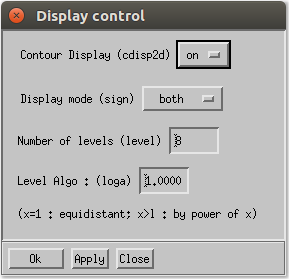
\includegraphics[width=0.5\textwidth]{figure2c.png}
\caption{The form resulting from the execution of the macro in Listing 1
is a static graphic box with an action button `Apply', with which the
macro command \texttt{dispcont\_doit} (\emph{not show}) is associated.}
\end{figure}

Slight differences can be observed between the original figures and the
current ones. Most of the differences come to simple improvements in the
program after the initial release, for instance the button `Cancel'
changed to `Close', or the reorganisation, and extension of the user
menus.

\begin{figure}
\centering
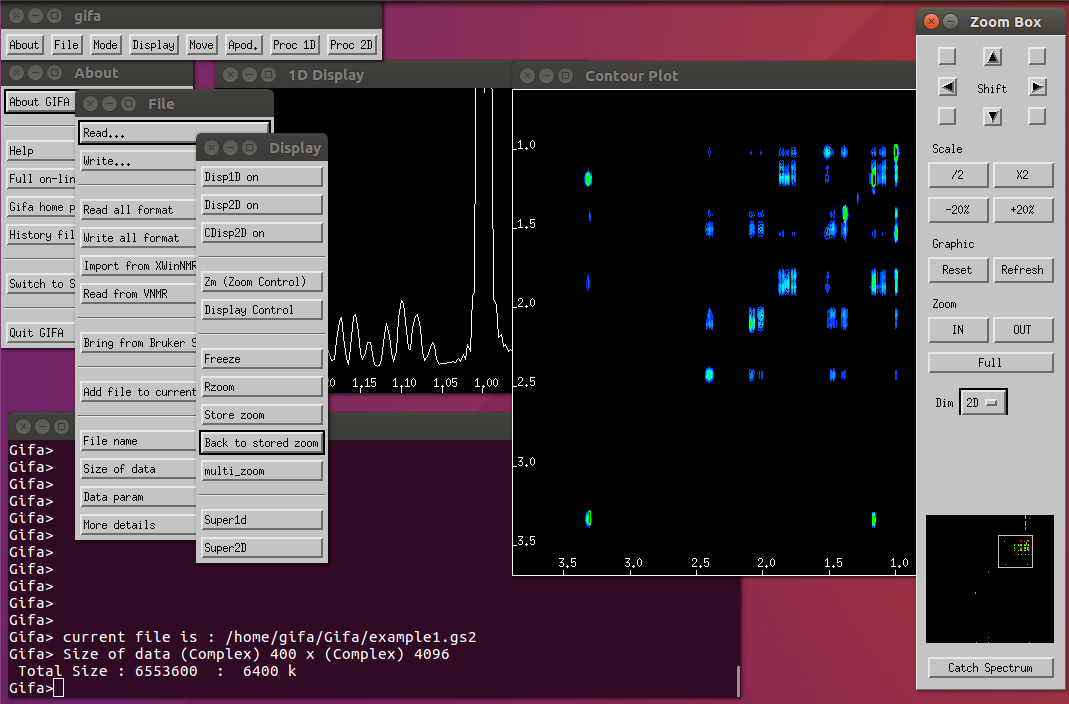
\includegraphics[width=0.99\textwidth]{figure3.png}
\caption{The default graphic environment as invoked during start-up of
Gifa. All the basic commands can be run from this graphic environment.
The control box called \texttt{Zoom\ Box} permits interaction with the
graphic window. The data are currently displayed in a contour plot 2D
window and in a 1D window. The small vignette seen in the
\texttt{Zoom\ Box} is a view of the complete data set held into the 2D
buffer, the square in it indicates the current zoom window.}
\end{figure}

The benchmark programs proposed in the original publication were run,
the results are shown in Table 1.

\begin{table}[h]
\centering
  \caption{Different processing times observed using the \emph{Gifa}
program \emph{(see reference \cite{Pons_1996} for details)} }
\begin{tabular}[]{@{}cccccc@{}}
\hline
Processing Time (s) & SUN & IBM & SGI & HP & This study\tabularnewline
\hline
2D & 17.5 & 12.6 & 10.5 & 7.5 & 0.05\tabularnewline
3D & 1064 & 329 & 193 & 172 & 1.10\tabularnewline
\hline
\end{tabular}
\end{table}

At this stage, the reproduction is considered as successful, even though
a complete check of all functionalities has not been fully performed.

\hypertarget{conclusion}{%
\section{Conclusion}\label{conclusion}}

The \emph{Gifa} program was successfully reproduced, in a relatively easy manner
for a software of this size, developed about 25 years ago.
The version of the code originally published was lost, but a later version of
the program was used and fully reproduced on a recent computer.
The reproduction was performed in a simple Virtual Machine, running the
32\ bit version of Ubuntu 16.04, which should be supported until April
2024.

The ease of porting is mostly coming from the use of standard tools and
programming languages, still well supported today (\texttt{f2c},
\texttt{perl}, \texttt{make}, \texttt{gzip}, \texttt{tar}, \ldots{}).
The program is one large code with very little external dependencies, as
it internally contains all mathematical routines, an internal macro
language, and its own GUI system. The only external libraries which had
to be installed are the X/Motif graphic and the \texttt{gdbm} the GNU
simple database engine, both being still supported under Linux. Also,
the diversity of the Unix environment in the nineties, imposed the
development a robust production pipeline easy to modify and to tune,
which has been a valuable tool in this reproduction.
The needed corrections
mostly consisted in finding and installing the correct software packets or
libraries.
Some tools and some structures had to be modified because of obsolete constructs
(Netscape\texttrademark\ or HTML comments for instance!).

Reviving the \emph{Gifa} program was an interesting experience, it
reminded me the qualities - and flaws - of this program, and
let me appreciate the efficiency of a monolithic program, with a tight memory management and
an algorithmics optimized to the limited resources available 20 years
ago. Despite its limitations, such a program can still have many
applications today, for instance embedded in a larger environment.

This work also showed that a monolithic program, written with simple
standard tools, with little dependencies on the environment, is quite
easy to maintained and can see its life extended beyond 20 years.

